
%! program = pdflatex

\documentclass[12pt]{article}
\usepackage{amsmath}
\usepackage{natbib}
\usepackage{graphicx}
\usepackage{amssymb}
\usepackage{epstopdf}
\usepackage{float} % to keep the figures in place
\usepackage{placeins}

\usepackage{caption}
\usepackage{subcaption}
\usepackage{color}
%\usepackage{undertilde}
\usepackage{enumitem}
\newcommand{\cred}{ \color{red}}
\newcommand{\cgreen}{\color{green}}
\newcommand{\cblue}{\color{blue}}
\newcommand{\cmag}{\color{magenta}}
\newcommand{\bn}{\begin{enumerate}}
\newcommand{\en}{\end{enumerate}}
\newcommand{\bi}{\begin{itemize}}
\newcommand{\ei}{\end{itemize}}
\newcommand{\be}{\begin{eqnarray}}
\newcommand{\ee}{\end{eqnarray}}
\newcommand{\by}{\begin{eqnarray*}}
\newcommand{\ey}{\end{eqnarray*}}
\renewcommand{\labelenumi}{(\alph{enumi}) }

\usepackage[margin=2.2cm, includehead]{geometry}% see geometry.pdf on how to lay out the page. There's lots.
\geometry{letterpaper} % or letter or a5paper or ... etc
% \geometry{landscape} % rotated page geometry
%\bibpunct{(}{)}{;}{a}{,}{,}
%\setlength{\textwidth}{16cm}
%\setlength{\textheight}{21cm}
\def\nonumber{\global\@eqnswfalse}
\newcounter{parnum}
\newcommand{\N}{%
  \noindent\refstepcounter{parnum}%
   \makebox[\parindent][l]{\textbf{[\arabic{parnum}]}}\quad  }
% Use a generous paragraph indent so numbers can be fit inside the
% indentation space.
\setlength{\parindent}{1.5em}

% See the ``Article customise'' template for come common customisations

\date{}
%\date{} % delete this line to display the current date

%%% BEGIN DOCUMENT
\usepackage{Sweave}
\begin{document}
\Sconcordance{concordance:aua257HW3.tex:aua257HW3.Rnw:%
1 52 1 1 0 63 1 1 217 20 1 2 2 42 1 1 302 2 1 2 2 7 1 1 9 1 2 5 1 1 6 1 %
2 6 1 1 18 1 2 7 1 1 9 1 2 7 1 1 301 2 1 2 2 7 1 1 9 1 2 5 1 1 6 1 2 7 %
1 1 18 1 2 6 1 1 9 1 2 45 1 1 158 7 1}

%\large
%\maketitle
\newtheorem{thm}{Theorem}[section]
\newtheorem{cor}[thm]{Corollary}
\newtheorem{lem}[thm]{Lemma}
\newtheorem{prop}[thm]{Proposition}
\newtheorem{defn}[thm]{Definition}
\newtheorem{exam}[thm]{Example}
\newtheorem{qstn}[thm]{Question}

%%%
\newpage
\begin{center}
{\bf Homework 3 - STAT 540}\\
Amal Agarwal
\end{center}
%==========================
\section*{Answer 1}
\begin{enumerate}[label=(\alph*)]
\item
\begin{enumerate}[label=(\roman*)]
\item Psudocode for Nelder-Mead simplex algorithm:
\begin{itemize}
\item Initialization: Since the maximization of the log-likelihood function is over a three-dimensional space ($\mu, \xi, \sigma$), we minimize the negative log-likelihood function and start with an initial simplex S containing 4 vertices ($x_0, x_1, x_2, x_4$) such that $x_i \in \mathbb{R}^3$.
\item Iterations: Repeat the following steps till termination condition is satisfied.
\begin{itemize}
\item Ordering: In the current working simplex S, determine the indices $h,s,l$ of the worst, second worst and the best vertex, such that
\[f_h=\max_{j}f_j, f_s=\max_{j\neq h}f_j, f_l=\min_{j\neq h}f_j\]
\item Calculate the centroid c of the best side which is the one opposite to the worst vertex as $c:=\dfrac{1}{n}\sum_{j\neq h}x_j$
\item Transformation: Compute the new working simplex from the current one. First, replace only the worst vertex $x_h$ with a better point by using reflection, expansion or contraction with respect to the best side. All test points lie on the line defined by $x_h$ and $c$ , and at most two of them are computed in one iteration. If this succeeds, the accepted point becomes the new vertex of the working simplex. If this fails, shrink the simplex towards the best vertex $x_l$ . In this case, $n$ new vertices are computed. Simplex transformations in the Nelder-Mead method are controlled by four parameters satisfying the following constraints: $\alpha>0,0<\beta<1,\gamma>1,\gamma>\alpha,0<\delta<1$.

\begin{itemize}
\item Reflect: Compute the reflection point $x_r:=c+\alpha(c-x_h)$ and $f_r:=f(x_r)$. If $f_l\leq f_r<f_s$ , accept $x_r$ and terminate the iteration.
\item Expand: If $f_r<f_l$ , compute the expansion point $x_e:=c+\gamma(x_r−c)$ and $f_e:=f(x_e)$ . If $f_e<f_r$ , accept $x_e$ and terminate the iteration. Otherwise (if $f_e \geq f_r$), accept $x_r$ and terminate the iteration.
\item Contract: If $f_r\geq f_s$ , compute the contraction point $x_c$ by using the better of the two points $x_h$ and $x_r$.
\begin{itemize}
\item Outside: If $f_s\leq f_r<f_h$ , compute $x_c:=c+\beta(x_r-c)$ and $f_c:=f(x_c)$. If $f_c\leq f_r$, accept $x_c$ and terminate the iteration.
Otherwise, perform a shrink transformation.
\item Inside: If $f_r\geq f_h$ , compute $x_c:=c+\beta(x_h-c)$ and $f_c:=f(x_c)$ . If $f_c<f_h$ , accept $x_c$ and terminate the iteration.
\end{itemize}
Otherwise, perform a shrink transformation.
\item Shrink: Compute $n$ new vertices $x_j:=x_l+\delta(x_j-x_l)$ and $f_j:=f(x_j)$, for $j=0,...,n$, with $j\neq l$ .
\end{itemize}
\end{itemize}
\item Termination: When the working simplex S is sufficiently small in some sense i.e. some or all vertices $x_j$ are close enough, terminate the algorithm.
\end{itemize}
(Reference: Scholarpedia)
\item Psudocode for Newton- Raphson algorithm:
\begin{itemize}
\item Start with an initial value $x^{(0)}=(\mu^{(0)},\xi^{(0)},\sigma^{(0)})$
\item Run loop until the termination condition is satisfied.
\begin{itemize}
\item $x^{(t+1)}=x^{(t)}-\nabla^2 l(x^{(t)}) \times \nabla l(x^{(t)})$ where $\nabla l(x^{(t)})$ is the gradient of log likelihood function evaluated at the the iterate $x^{(t)}=(\mu^{(t)},\xi^{(t)},\sigma^{(t)})$ and $\nabla^2 l(x^{(t)})$ is the hessian of log likelihood function evaluated at the the iterate $x^{(t)}=(\mu^{(t)},\xi^{(t)},\sigma^{(t)})$.
\item Check if $|x^{(t+1)}-x^{(t)}|<tol$ to terminate the loop. Here tol is some pre-specified tolerance.
\end{itemize}
\end{itemize}
 

\item Choosing the initial values: For both the above algorithms along with BFGS, the built-in function optim in R was used to calculate the MLE of ($\mu, \zeta, \sigma$) for the given data. In optim the initial values were passed as the maximizers of the log likelihood function over a grid of $1000$ points in the 3-dimensional parameter space. The end-points of the grid were randomly chosen as $(1,5)\times(0.1,5)\times(0.05,5.5)$.
\end{enumerate}

\item The following table gives the required information:
\begin{table}[H]
\centering
\caption{ML estimates and standard errors for the three algorithms}
\label{my-label}
\begin{tabular}{|c|c|c|}
\hline
               & ML estimates for ($\mu, \xi, \sigma$)& Standard errors for ($\mu, \xi, \sigma$)\\ \hline
BFGS           &(1.65,0.18,0.098)&(0.0021,0.0205,0.0017)\\ \hline
Nelder-Mead    &(1.65,0.18,0.098)&(0.0021,0.0205,0.0017)\\ \hline
Newton Raphson &(1.65,0.18,0.098)&(0.0021,0.0205,0.0017)\\ \hline
\end{tabular}
\end{table}

Standard error estimates of ($\mu, \xi, \sigma$) were found by inverting the observed information matrix and taking the square root of the diagnol entries which correspond to ($\mu, \xi, \sigma$) respectively. This is using the asymptotic theory for MLE's which gives the following convergence in law.
\[\sqrt{n}(\hat{\theta_n}-\theta)\longrightarrow N(0, I^{-1}(\theta))\]
Now we know that the observed information is the negative of the Hessian matrix. For the first two algorithms BFGS and Nelder-Mead, the negative Hessian matrix can be extracted from the optim function. For the Newton-Raphson algorithm, the Hessian matrix was computed for the last iterate using "hessian" function from the package "pracma". Note that in all the above cases the observed information is for the whole dataset (not just one data point) and so division by $n$ is not required. 

\item The following figure gives the fitted GEV density for all the three optimization algorithms over histogram of the data. 

\begin{figure}[H]
\begin{centering}
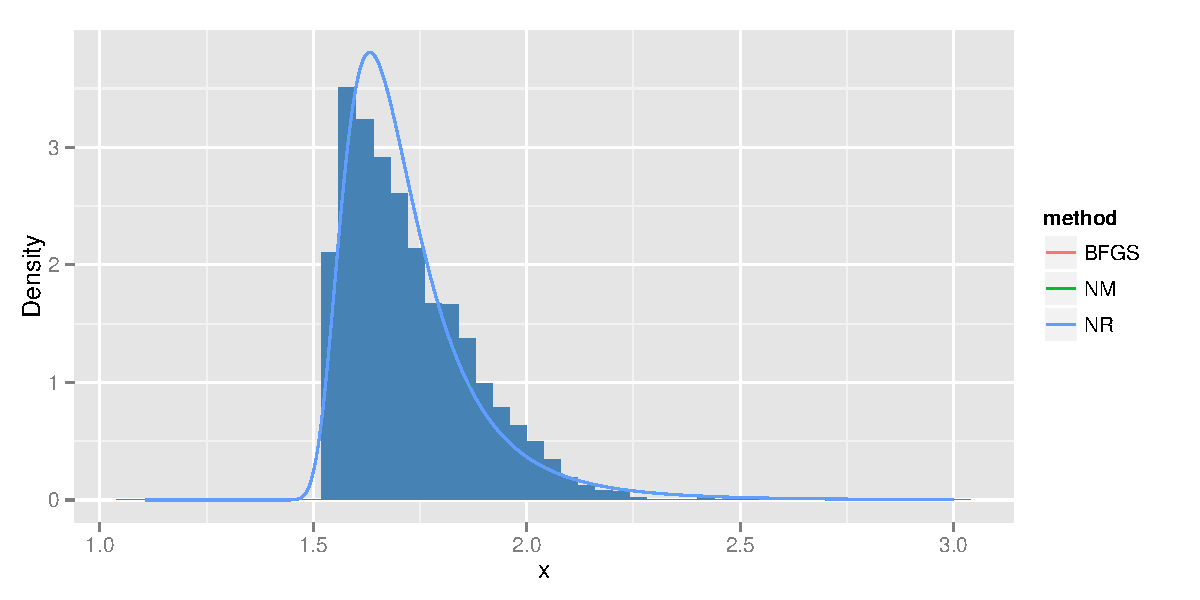
\includegraphics{aua257HW3-002}
\caption{Plot of fitted density for three algorithms over the histogram of the data}
\end{centering}
\end{figure}
Clearly the lines seem to coincide which shows that the parameter estimates are really close.
\end{enumerate}

%%%%%%%%%%%%%%%%%%%%%%%%%%%%%%%%%%%%%%%%%%%%%%%%%%%%%%%%%%%%%%%%%%%%%%%%%%%%%%%%%%%%
\section*{Answer 2}
\begin{enumerate}[label=(\alph*)]
\item 
\begin{enumerate}[label=(\roman*)]
\item
Pseudocode for the first Metropolis Hastings algorithm (Variable one at a time) for the given target density:
\begin{itemize}
\item Start off with $x^{0}=(\mu^{(0)},\xi^{(0)},\sigma^{(0)})$ chosen suitably after a series of pilot runs. Choose the length of the Markov chain as $m$.
\item Run loop from $t=0:(m-1)$
\begin{itemize}
\item Assign the current state as $x^{(t)}=(\mu^{(t)},\xi^{(t)},\sigma^{(t)})$.
\item Generate a candidate $\mu^{*}$ drawn from univariate normal distribution with mean as $\mu^{(t)}$ and variance $\tau_{\mu}^2$ being the tuning parameter.
\item Accept $\mu^{*}$ as next state $\mu^{(t+1)}$ with the following acceptance probability $\alpha_\mu$, else assign the current state as next state.
\[\alpha_\mu(\mu^{*},\mu^{(t)})=\text{min}\left(1,\dfrac{h_{\mu}(\mu^{*},\xi^{(t)},\sigma^{(t)})q_\mu(\mu^{*},\mu^{(t)})}{h_\mu(\mu^{(t)},\xi^{(t)},\sigma^{(t)})q_\mu(\mu^{(t)},\mu^{*})}\right)=\text{min}\left(1,\dfrac{h_\mu(\mu^{*},\xi^{(t)},\sigma^{(t)})}{h_\mu(\mu^{(t)},\xi^{(t)},\sigma^{(t)})}\right)\]
where $h_\mu$ is the conditional target kernel for $\mu$ which the product of the likelihood function and the uniform prior (contains no term for the given prior) and $q_\mu$ is univariate normal proposal density which cancels out being symmetric.

\item Generate a candidate $\xi^{*}$ drawn from univariate normal distribution with mean as $\xi^{(t)}$ and variance $\tau_{\xi}^2$ being the tuning parameter.
\item Accept $\xi^{*}$ as next state $\xi^{(t+1)}$ with the following acceptance probability $\alpha_\xi$, else assign the current state as next state.
\[\alpha_\xi(\xi^{*},\xi^{(t)})=\text{min}\left(1,\dfrac{h_\xi(\mu^{(t+1)},\xi^{*},\sigma^{(t)})q_\xi(\xi^{*},\xi^{(t)})}{h_\xi(\mu^{(t+1)},\xi^{(t)},\sigma^{(t)})q_\xi(\xi^{(t)},\xi^{*})}\right)=\text{min}\left(1,\dfrac{h_\xi(\mu^{(t+1)},\xi^{*},\sigma^{(t)})}{h_\xi(\mu^{(t+1)},\xi^{(t)},\sigma^{(t)})}\right)\]
where $h_\xi$ is the conditional target kernel for $\xi$ which is the product of the likelihood function and the uniform prior (contains no term for the given prior) and $q_\xi$ is univariate normal proposal density which cancels out being symmetric.

\item Generate a candidate $\sigma^{*}$ drawn from univariate truncated normal distribution with bounds as $(0,\infty)$. Again take the mean of this proposal as $\sigma^{(t)}$ and variance as $\tau_{\sigma}^2$ being the tuning parameter.
\item Accept $\sigma^{*}$ as next state $\sigma^{(t+1)}$ with the following acceptance probability $\alpha_\sigma$, else assign the current state as next state.
\[\alpha_\sigma(\sigma^{*},\sigma^{(t)})=\text{min}\left(1,\dfrac{h_\sigma(\mu^{(t+1)},\xi^{(t+1)},\sigma^{*})q_\sigma(\sigma^{*},\sigma^{(t)})}{h_\sigma(\mu^{(t+1)},\xi^{(t+1)},\sigma^{(t)})q_\sigma(\sigma^{t},\sigma^{*})}\right)\]
where $h_\sigma$ is the conditional target kernel for $\sigma$ which is the product of the likelihood function and the uniform prior and $q_\sigma$ is univariate truncated normal proposal density.

\item Assign the next state as $x^{(t+1)}=(\mu^{(t+1)},\xi^{(t+1)},\sigma^{(t+1)})$.
\end{itemize}
\end{itemize}
\item Pseudocode for the second Metropolis Hastings algorithm (Variable one at a time) for the given target density is same as the first one above with just the change in proposal density $q_\sigma$ for $\sigma$ as gamma density instead of univariate truncated normal. The mean of $q_\sigma$ is chosen as the current state and the variance is kept as the tuning parameter.
\item As before, starting values for both the algorithms were chosen as the maximizers of the log likelihood function over a grid of $1000$ points in the 3-dimensional parameter space. The end-points of the grid were randomly chosen as $(1,5)\times(0.1,5)\times(0.05,5.5)$.
\end{enumerate}
\item For both the algorithms, the appropriate chain length was chosen as $2500$ since the all the diagnostics shown below suggest that the convergence takes place till after this point. Besides, the relative error i.e. the ratio of MCMC standard error to the estimate drops below $10^{-2}$ for $n>2500$ which is reasonably good. 
\clearpage
\begin{enumerate}[label=(\roman*)]
\item Diagnostics for algorithm 1:
Plot of the ACF of samples is given as:
\begin{figure}[H]
\begin{centering}
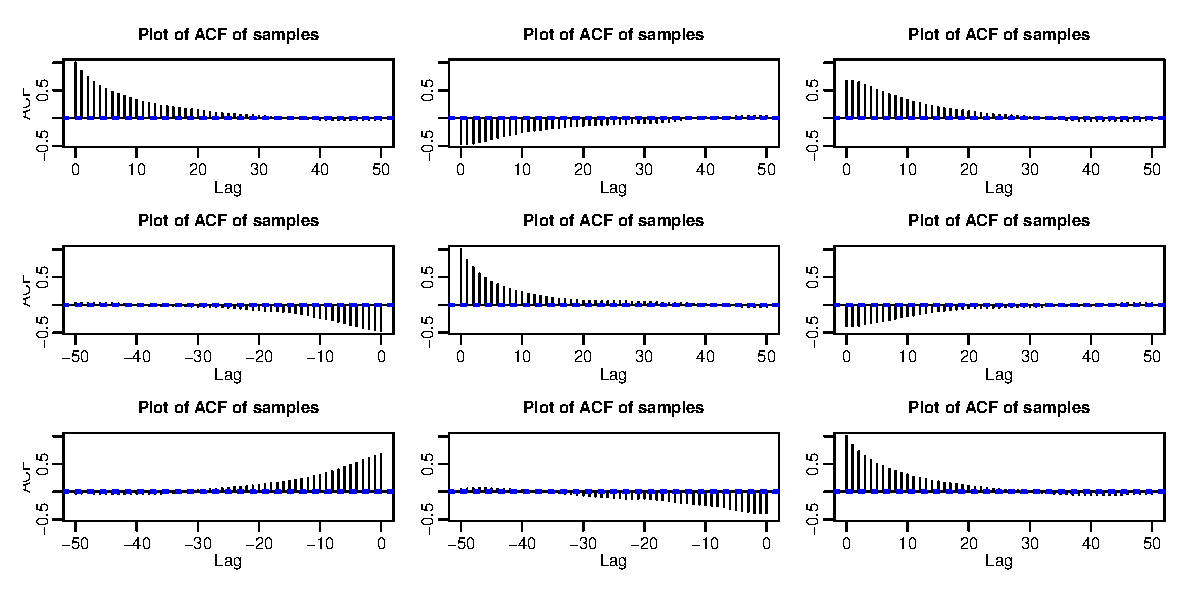
\includegraphics{aua257HW3-004}
\caption{Plot of ACF of samples}
\end{centering}
\end{figure}
For all the 3 components, the above plot is reasonably good which indicates that the tuning parameter value of $(4.36\times 10^{-6}, 4.20\times 10^{-4}, 2.88\times 10^{-6})$ may not be the best but still it works reasonably good.

For 3 different starting values as (1.65,0.17,0.098), (1.64,0.18,0.091) and (1.65,0.17,0.127), labelled as $1$, $2$ and $3$, plots of estimates of expected values of $(\mu,\xi,\sigma)$ and Monte Carlo standard errors with sample size are given below:
\begin{figure}[H]
\begin{centering}
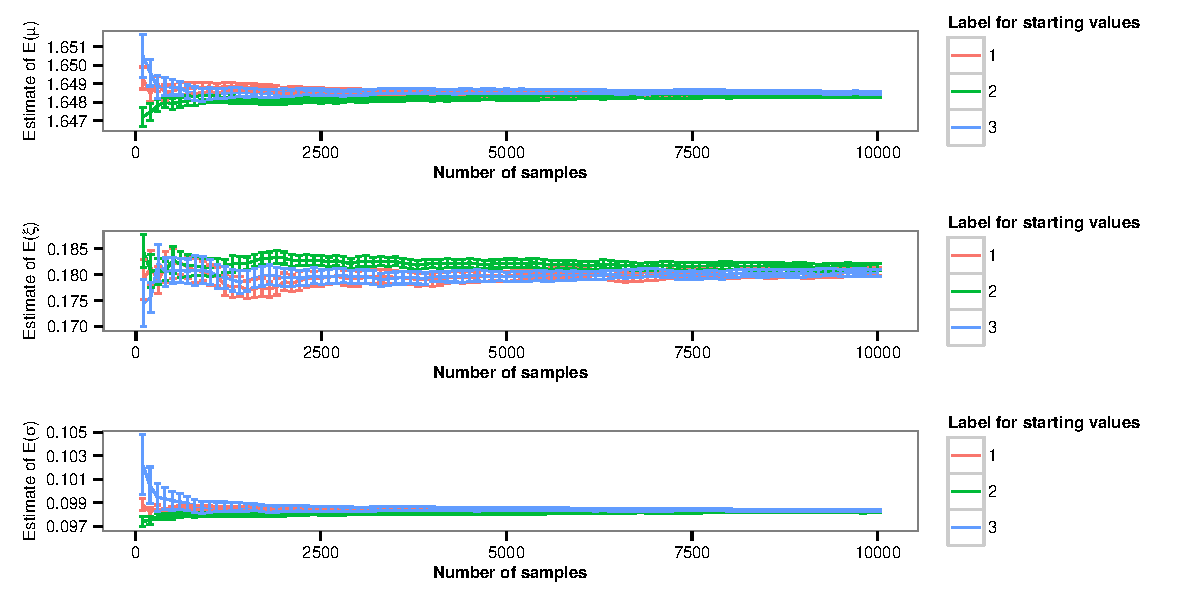
\includegraphics{aua257HW3-005}
\caption{Plot of estimates vs. sample size with error bars for $(\mu,\xi,\sigma)$}
\end{centering}
\end{figure}

\begin{figure}[H]
\begin{centering}
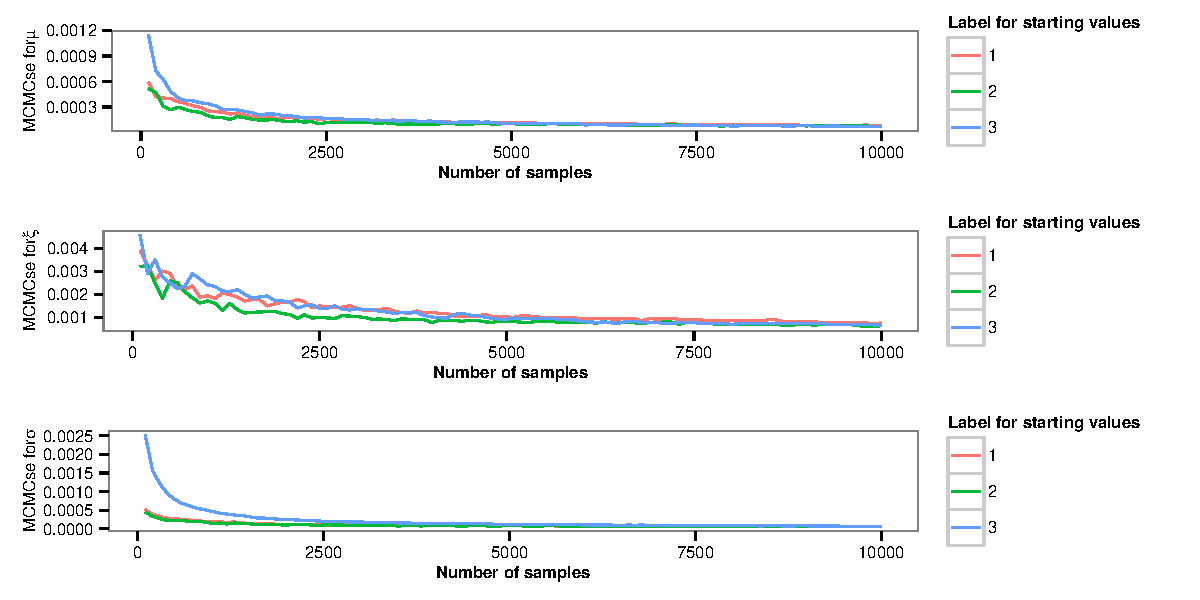
\includegraphics{aua257HW3-006}
\caption{Plot of MCMC se vs. sample size for $(\mu,\xi,\sigma)$}
\end{centering}
\end{figure}
The above plots show that for all the 3 components and for different starting alues, the estimates converge to same value and MCMC standard errors converge to 0. This verifies the algorithm to some extent.
Plotting the estimated density after $n/2$ and after $n$:
\begin{figure}[H]
\begin{centering}
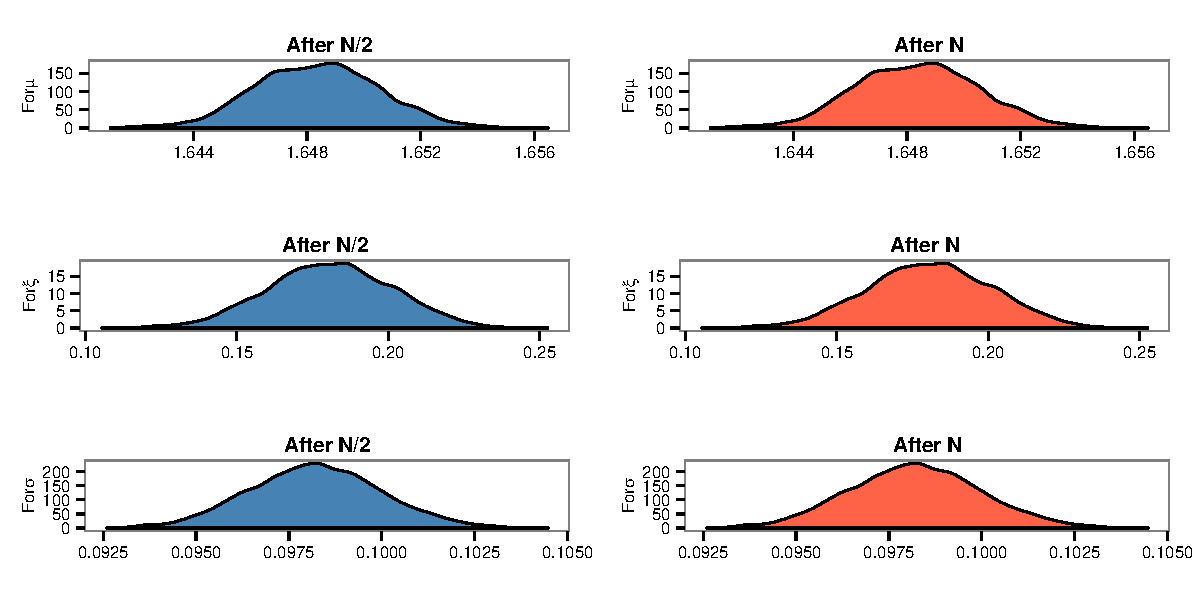
\includegraphics{aua257HW3-007}
\caption{Plot of estimated density for $(\mu,\xi,\sigma)$ after N/2 and N}
\end{centering}
\end{figure}
\clearpage

Plotting the estimated density for different starting values for all the components:
\begin{figure}[H]
\begin{centering}
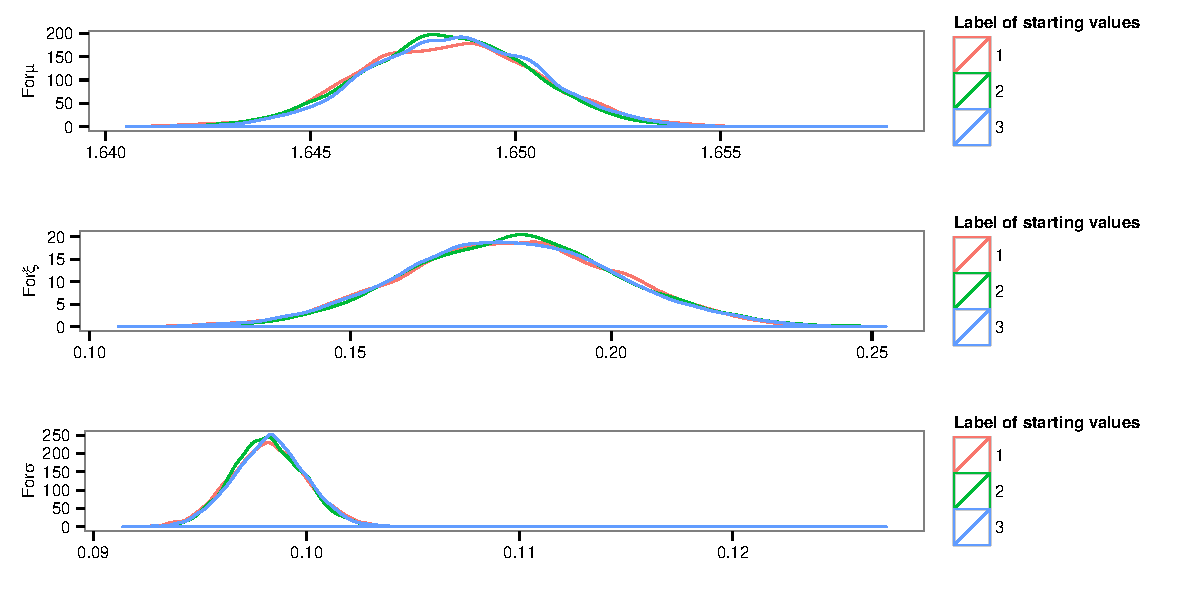
\includegraphics{aua257HW3-008}
\caption{Plot of marginal density for $(\mu,\xi,\sigma)$}
\end{centering}
\end{figure}
From the above plots, the estimated densities after $n/2$ and after $n$ look reasonably identical for all the 3 components. Also the estimated density for different starting values also overlap to a good extent. This further verifies the robustness and convergence of the algorithm.

%%%%%%%%%%%%%%%%%%%%%%%%%%%%%%%%%%%%%%%%

\item Diagnostics for algorithm 2:
Plot of the ACF of samples is given as:
\begin{figure}[H]
\begin{centering}
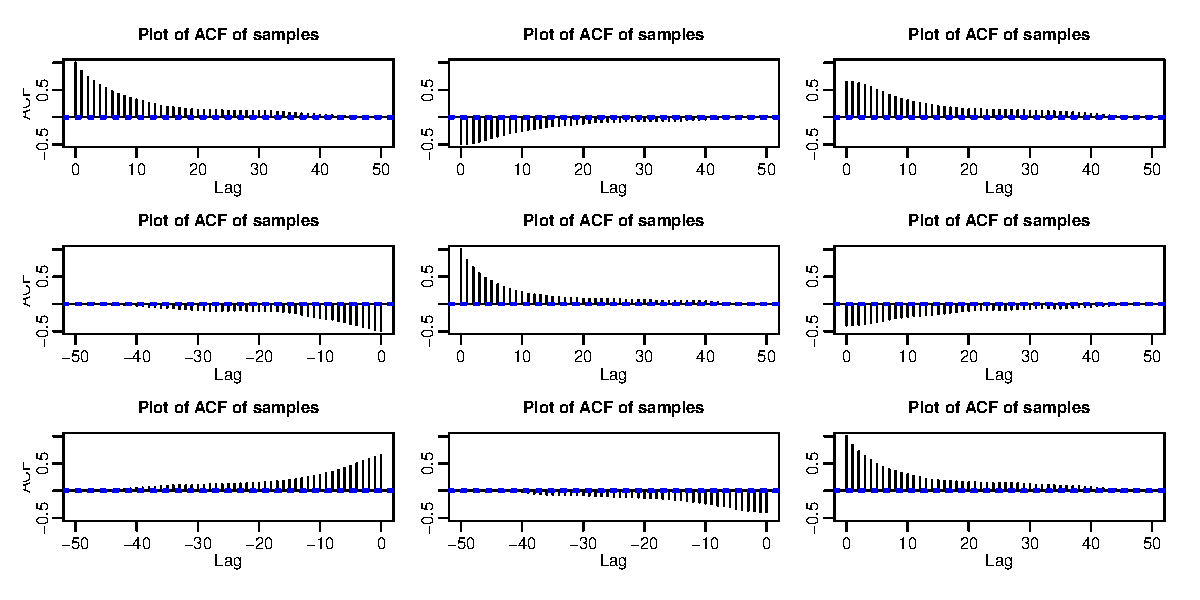
\includegraphics{aua257HW3-010}
\caption{Plot of ACF of samples}
\end{centering}
\end{figure}
For all the 3 components, the above plot is reasonably good which indicates that the tuning parameter values of $(4.46\times 10^{-6}, 4.33\times 10^{-4}, 2.94\times 10^{-6})$ may not be the best but still it works reasonably good.

For 3 different starting values as (1.65,0.17,0.098), (1.62,0.16,0.102) and (1.68,0.2,0.093), labelled as $1$, $2$ and $3$, plots of estimates of expected values of $(\mu,\xi,\sigma)$ and Monte Carlo standard errors with sample size are given below:
\begin{figure}[H]
\begin{centering}
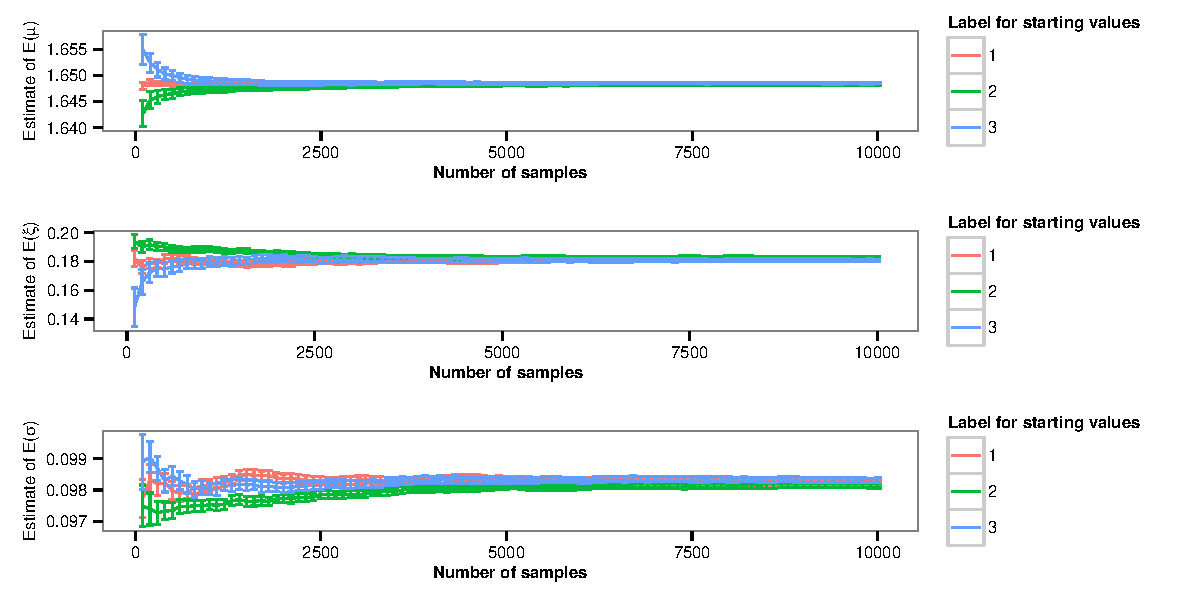
\includegraphics{aua257HW3-011}
\caption{Plot of estimates vs. sample size with error bars for $(\mu,\xi,\sigma)$}
\end{centering}
\end{figure}

\begin{figure}[H]
\begin{centering}
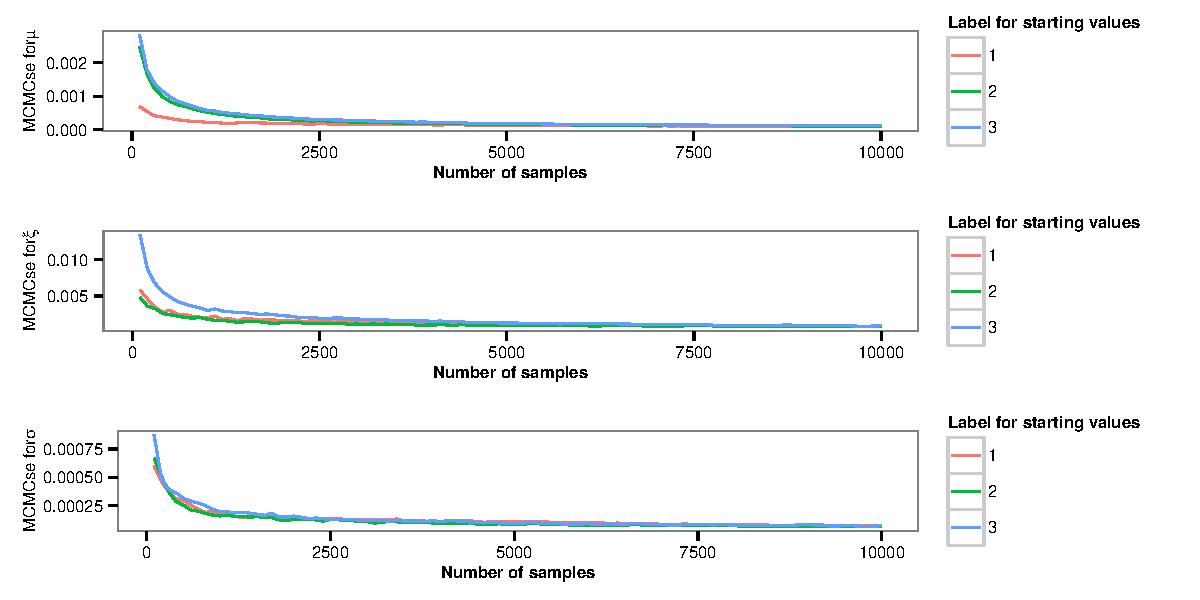
\includegraphics{aua257HW3-012}
\caption{Plot of MCMC se vs. sample size for $(\mu,\xi,\sigma)$}
\end{centering}
\end{figure}
The above plots show that for all the 3 components and for different starting alues, the estimates converge to same value and MCMC standard errors converge to 0. This verifies the algorithm to some extent.
\clearpage
Plotting the estimated density after $n/2$ and after $n$:
\begin{figure}[H]
\begin{centering}
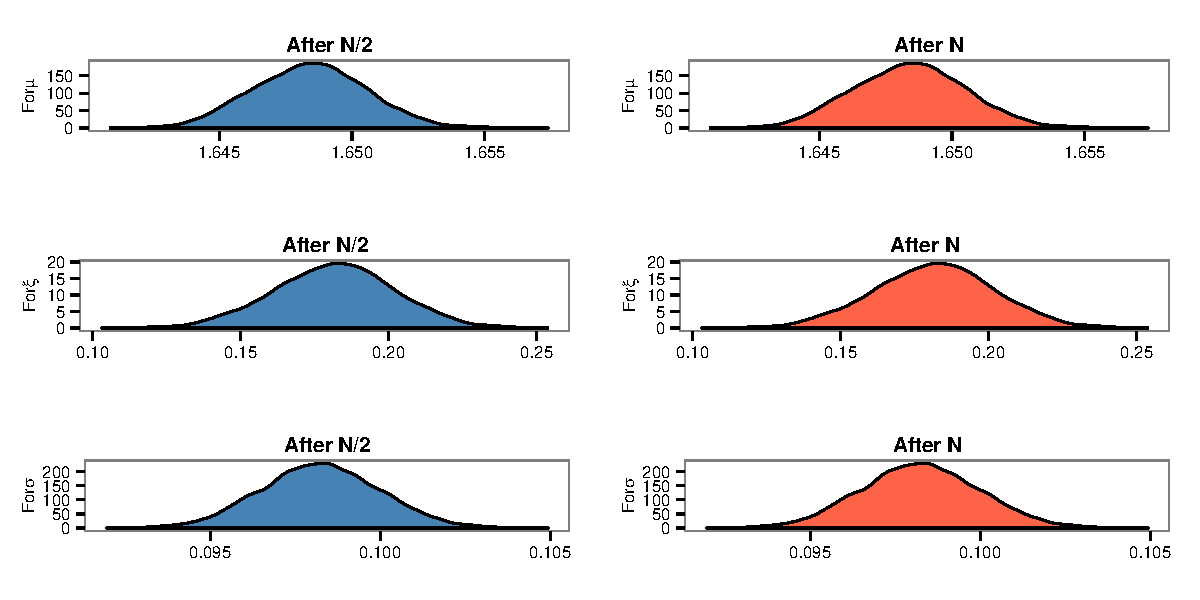
\includegraphics{aua257HW3-013}
\caption{Plot of estimated density for $(\mu,\xi,\sigma)$ after N/2 and N}
\end{centering}
\end{figure}

Plotting the estimated density for different starting values for all the components:
\begin{figure}[H]
\begin{centering}
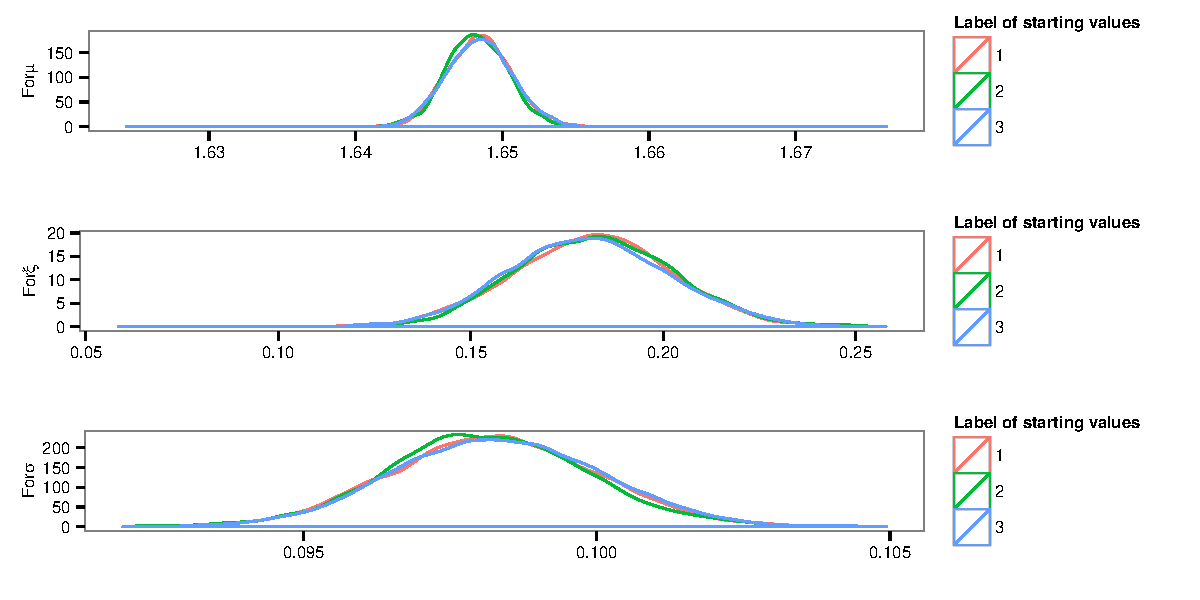
\includegraphics{aua257HW3-014}
\caption{Plot of marginal density for $(\mu,\xi,\sigma)$}
\end{centering}
\end{figure}
From the above plots, the estimated densities after $n/2$ and after $n$ look reasonably identical for all the 3 components. Also the estimated density for different starting values also overlap to a good extent. This further verifies the robustness and convergence of the algorithm.
\end{enumerate}

\clearpage
\item The following table gives the required information:
\begin{table}[H]
\centering
\caption{Posterior estimates, standard deviations and MCMC standard errors}
\label{my-label}
\begin{tabular}{|c|c|c|c|}
\hline
            & Posterior estimates for $(\mu,\xi,\sigma)$ & MCMC standard errors & Posterior standard deviations \\ \hline
Algorithm 1 & (1.65, 0.18, 0.098) &(4e-04, 0.0026, 3e-04)& (0.0022, 0.0208, 0.0018)\\ \hline
Algorithm 2 &(1.65, 0.18, 0.098) &(4e-04, 0.0034, 4e-04)&(0.0022, 0.0208, 0.0018)\\ \hline
\end{tabular}
\end{table}

\item The following table gives the required information:

\begin{table}[H]
\centering
\caption{Comparing confidence and credible intervals for different algorithms}
\label{my-label}
\begin{tabular}{|c|c|c|c|}
\hline
               & Conf. int. for $\mu$ & Conf. int. for $\xi$ & Conf. int. for $\sigma$ \\ \hline
BFGS           &(1.6442, 1.6525)&(0.1407, 0.2212)&(0.0948, 0.1015) \\ \hline
Nelder-Mead    &(1.6442, 1.6525)  &(0.1406, 0.221)   & (0.0948, 0.1015)\\ \hline
Newton Raphson &(1.6442, 1.6524)  &(0.1408, 0.2212) &(0.0948, 0.1015)\\ \hline
               &Cred. int. for $\mu$ & Cred. int. for $\xi$ & Cred. int. for $\sigma$ \\ \hline
Algorithm 1    &(1.6441, 1.6526)&(0.1396, 0.2204)&(0.0948, 0.1018)\\ \hline
Algorithm 2    &(1.6443, 1.6527)&(0.1403, 0.2216)&(0.0948, 0.1017)\\ \hline
\end{tabular}
\end{table}

\end{enumerate}

%%%%%%%%%%%%%%%%%%%%%%%%%%%%%%%%%%%%%%%%%%%%%%%%%%%%%%%%%%%%%%%%%%%%%%%%%%%%%%%%%%

\section*{Answer 3}
\begin{enumerate}[label=(\alph*)]
\item Among the three optimization algorithms, viz. BFGS, Nelder-Mead and Newton-Raphson, we observed earlier that the Newton Raphson algorithm does not converge if the initial values of the parameters $(\mu,\xi,\sigma)$ are not too close to the MLE's. Also, there is not any apparent difference between BFGS and Nelder-Mead algorithm since the standard errors are exactly same. Therefore best optimization algorithm to compute the MLE's was chosen randomly as Nelder-Mead. With the given parameters $1000$ data points were simulated for one set. The number of sets determine the Monte Carlo sample size.


For the three parameters $(\mu,\xi,\sigma)$, the estimates of mean square errors were obtained as (0.000945, 0.000883, 0.000684). The corresponding Monte-Carlo standard errors for these approximations were (0.000111, 9e-05, 6.2e-05).

\item The coverage probabilties for $95\%$ confidence intervals for $(\mu,\xi,\sigma)$ were obtained as (0.9536, 0.9588, 0.9485). The corresponding Monte-Carlo standard errors for these approximations were (0.0151, 0.0143, 0.0159).

\item The simulation study was carried out by generatng datasets one by one and calculating sample mean estimates and standard for all the three parameters using Nelder Mead algorithm. We define the relative error for each parameter as the ratio of Monte Carlo standard error to the point estimate (sample mean) upto a particular Monte Carlo sample size. The generation of datasets was stopped when the maximum of the relative error for all parameters becomes less than an arbitrary tolerance of $5 \times 10^{-3}$. The number of datasets chosen gives the Monte Carlo sample size of 194 for the chosen tolerance. Also at each iterate the log likelihood function was evaluated on a grid of $125$ points in the parameter space. For the first iterate, the grid end-points were initialized arbirarily at $(-10,10)\times (-10,10)\times (0.1,10.1)$. For the successive iterates, the grid end-points were fixed as the $95\%$ confidence bounds obtained in the previous iterate. Note that this approach to choose initial values exploits the information from successive simulated datasets, thereby making the estimates and standard errors more and more accurate as the number of iterations increase.
\end{enumerate}
\end{document}
